\section{Utilizzo plug-in}
    \subsection{Abilitazione plug-in}
        Dopo aver installato il plug-in nella piattaforma Grafana\glo, la prima cosa da fare è abilitarlo. È quindi necessario connettersi alla pagina principale di Grafana\glosp e successivamente bisogna:
        \begin{enumerate}
            \item dal menù laterale cliccare sulla voce "Plugins" dentro alla sezione "Configuration" (icona con l'ingranaggio);
            \item selezionare e cliccare l'app "Grafana prediction plugin";
            \item infine, nella pagina seguente (pagina di configurazione del plug-in), cliccare il pulsante "Enable".
        \end{enumerate}
        \begin{figure}[H]
            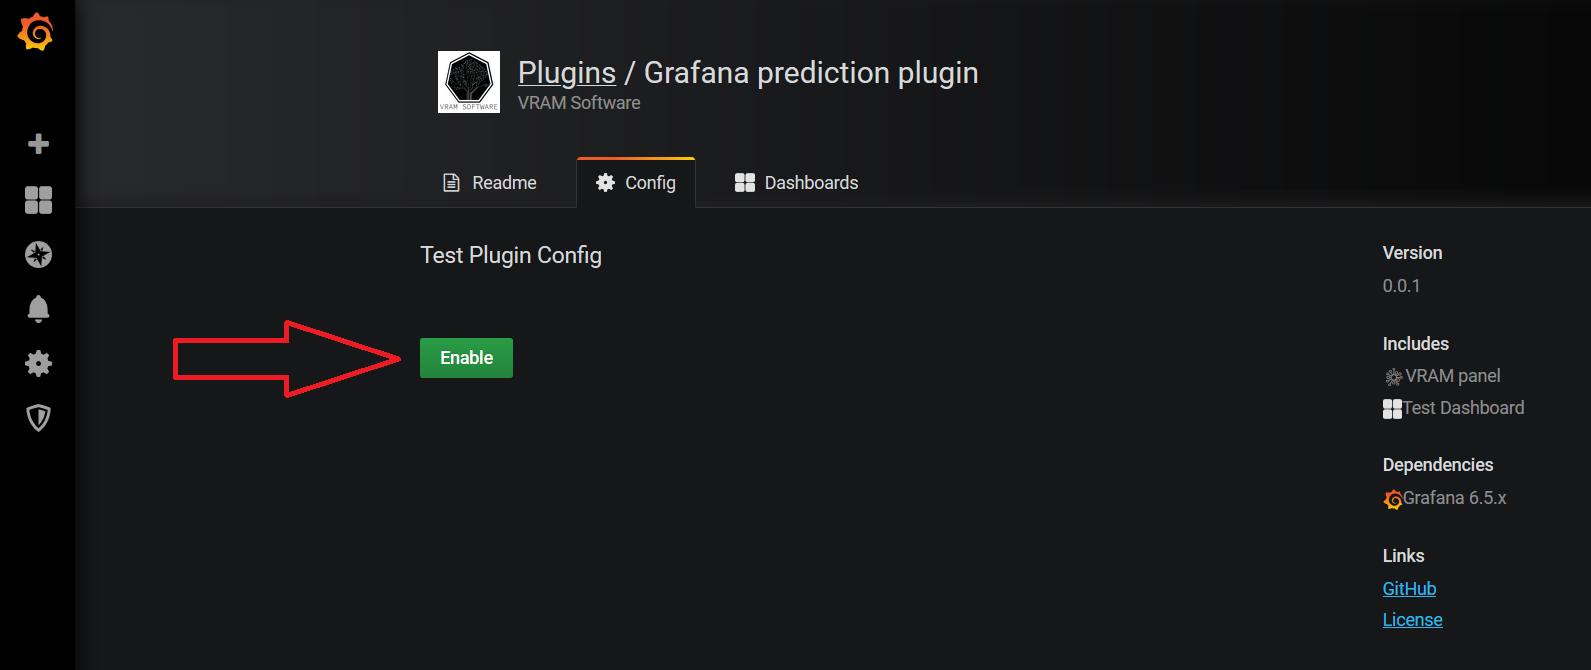
\includegraphics[width=\textwidth,height=\textheight,keepaspectratio]{img/abilitazione_plug-in.png}
            \caption{Pagina di configurazione del plug-in atta all'abilitazione.}
        \end{figure}
    \subsection{Aggiunta panel}
        Ad abilitazione avvenuta, la prima cosa da fare per interagire con il plug-in è aggiungere il pannello di \textit{VRAM Software} nella dashboard\glo. Per farlo bisogna seguire i seguenti passi:
        \begin{enumerate}
            \item dal menù laterale cliccare la voce "Dashboard" dentro alla sezione "Create" (simbolo "+");
            \item scegliere l'opzione "Choose Visualization" dal riquadro;
            \item infine selezionare il pannello "VRAM panel".
        \end{enumerate}
        \begin{figure}[H]
            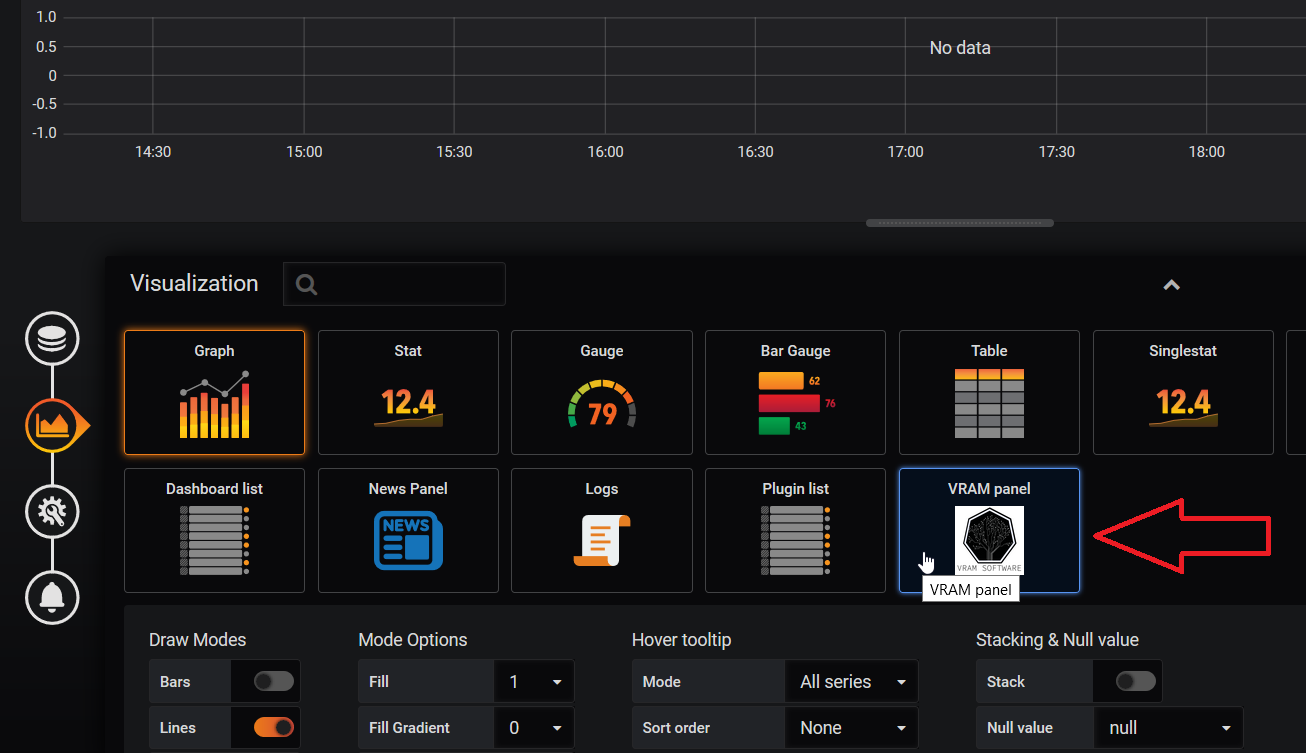
\includegraphics[width=\textwidth,height=\textheight,keepaspectratio]{img/aggiunta_plug-in.png}
            \caption{Pagina della scelta visualizzazione della dashboard\glo.}
        \end{figure}
    \subsection{Modificare il pannello}
        Una volta aggiunto il pannello sarà possibile modificare la sua configurazione. Per fare ciò si devono seguire i seguenti passaggi dalla homepage di Grafana\glo:
        \begin{enumerate}
            \item dal menù laterale cliccare sulla voce "Manage" dentro alla sezione "Dashboard" (icona con i quattro riquadri);
            \item cliccare il nome della dashboard\glosp a cui si vuole accedere (eventualmente usare i vari filtri offerti da Grafana\glosp per facilitare la ricerca);
            \item infine ci si troverà di fronte al grafico desiderato dove bastera premere sul nome e selezionare la voce "Edit".
        \end{enumerate}
        \begin{figure}[H]
            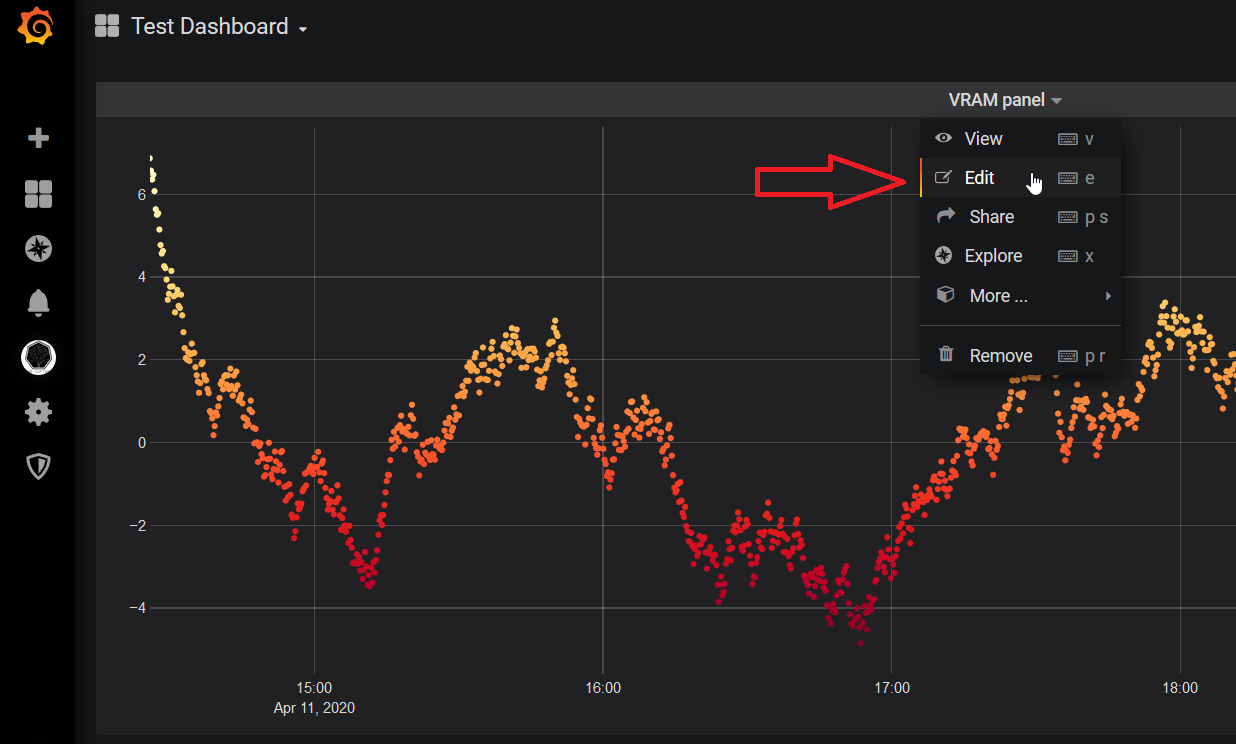
\includegraphics[width=\textwidth,height=\textheight,keepaspectratio]{img/modificare_pannello.png}
            \caption{Selezione opzioni pannello.}
        \end{figure}
        In alternativa, se la dashboard\glosp è stata usata recentemente, è possibile trovare il suo nome direttamente in homepage. Diventa quindi sufficiente seguire le istruzioni sopracitate dal punto numero 2.
    \subsection{Importazione e rimozione file JSON dei predittori}
        Nel pannello è possibile aggiungere un file JSON contenente i predittori\glosp precedentemente calcolati tramite l'applicativo esterno. Per farlo bisogna seguire i seguenti passi:
        \begin{enumerate}
            \item entrare nella sezione di modifica del pannello;
            \item nel menù laterale cliccare la voce "Visualization" (icona del grafico);
            \item nel riquadro "Import json file" cliccare il pulsante "Upload .json file";
            \item selezionare il file desiderato dal file chooser e premere "Apri".
        \end{enumerate}
        \begin{figure}[H]
            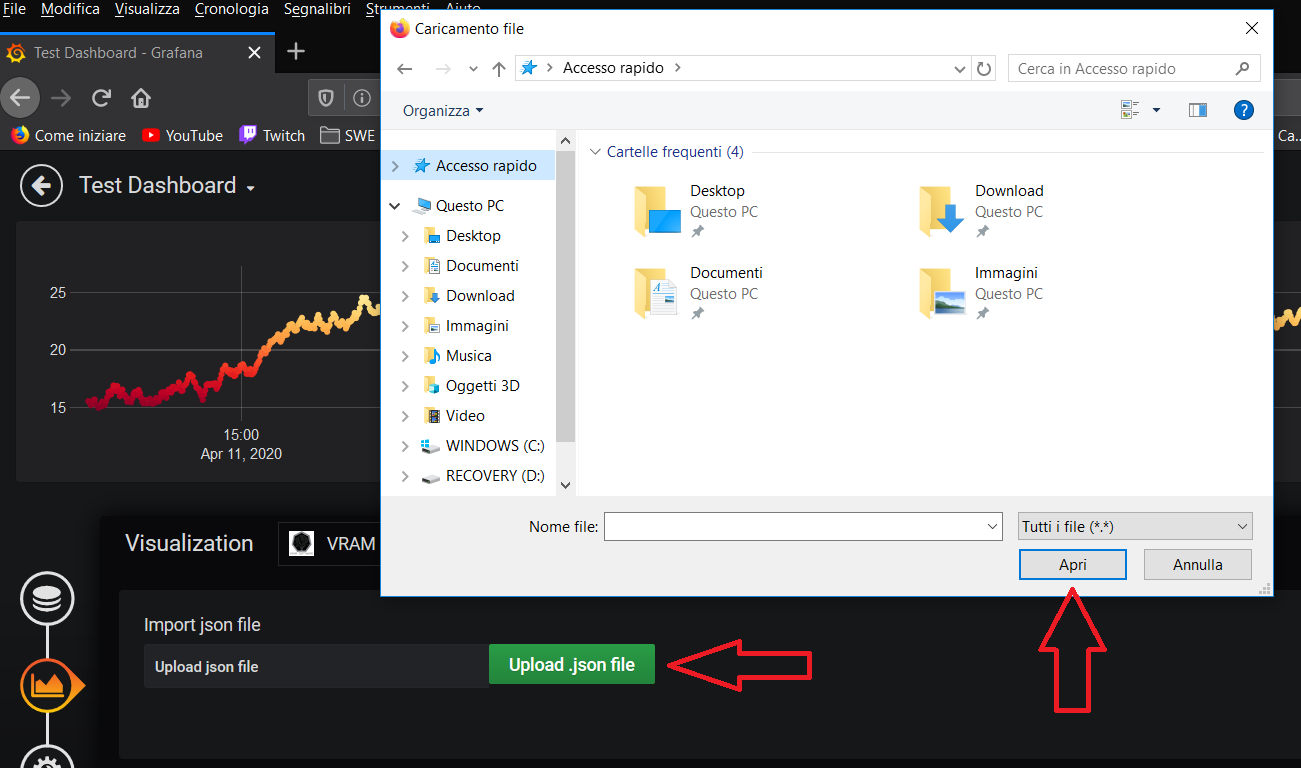
\includegraphics[width=\textwidth,height=\textheight,keepaspectratio]{img/importazione_e_rimozione_JSON.png}
            \caption{Riquadro "Import json file".}
        \end{figure}
        Caricato il file JSON sarà poi possibile rimuoverlo premendo sul pulsante "Remove" situato sempre nel riquadro "Import json file".
    \subsection{Associazione dei nodi al flusso dati}
        Se è stato caricato un file JSON valido, è possibile associare il flusso dati su Grafana\glosp ai predittori\glosp inseriti. Le istruzioni da seguire sono le seguenti:
        \begin{enumerate}
            \item entrare nella sezione di modifica del pannello;
            \item nel menù laterale cliccare la voce "Visualization" (icona del grafico);
            \item nel riquadro "Select query associations" saranno presenti delle label che indicano i predittori e dei selettori che permetteranno di scegliere il flusso dati desiderato;
            \item una volta scelta l'associazione per attuarla basterà premere il pulsante "Confirm".
        \end{enumerate}
        \begin{figure}[H]
            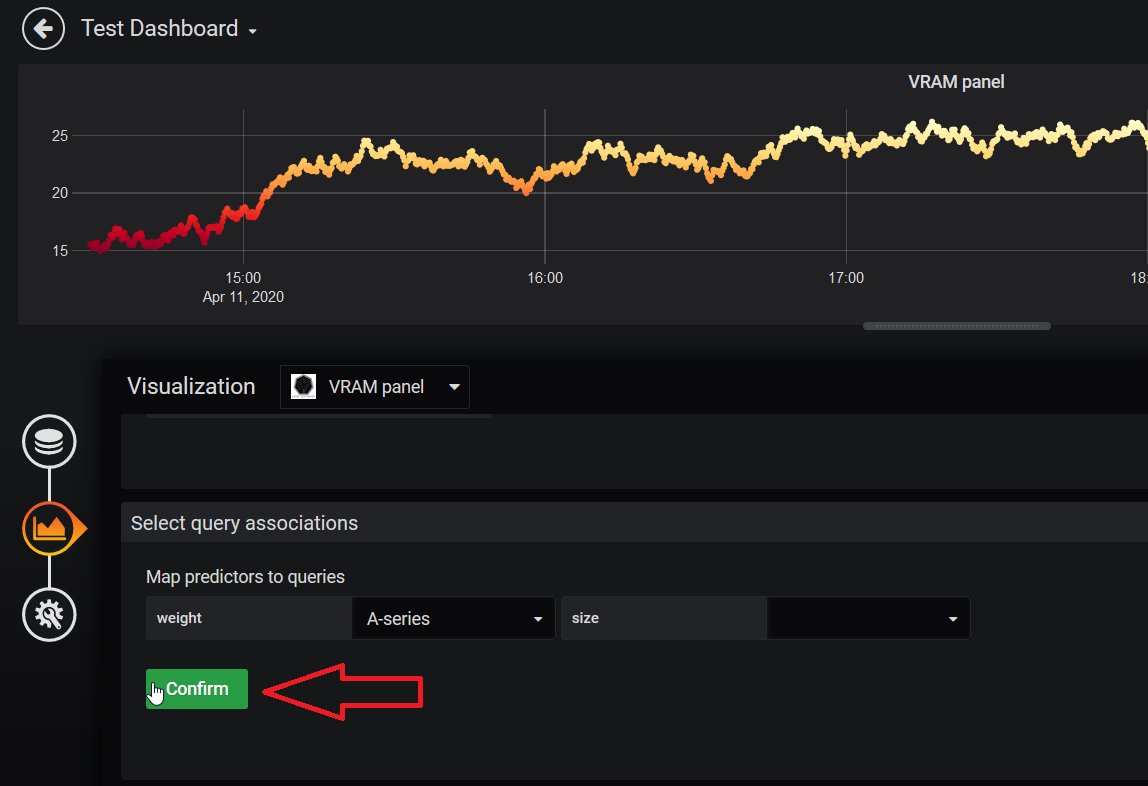
\includegraphics[width=\textwidth,height=\textheight,keepaspectratio]{img/associazione_nodi.png}
            \caption{Riquadro "Select query associations".}
        \end{figure}
    \subsection{Scrittura sul database InfluxDB}
        Se è stata configurata correttamente una datasource relativa ad un database InfluxDB, è possibile salvare i risultati della previsione. Per configurare la connessione col database InfluxDB bisogna:
        \begin{enumerate}
            \item entrare nella sezione di modifica del pannello;
            \item nel menù laterale cliccare la voce "Visualization" (icona del grafico);
            \item nel riquadro "Configure influxDB destination" bisogna inserire:
            \begin{enumerate}
                \item datasource (per ora è disponibile solo InfluxDB);
                \item nome del database;
                \item measurement;
                \item field key.
            \end{enumerate}
            \item una volta inseriti i dati basterà premere il tasto "Confirm" per convalidare il collegamento.
        \end{enumerate}
        \begin{figure}[H]
            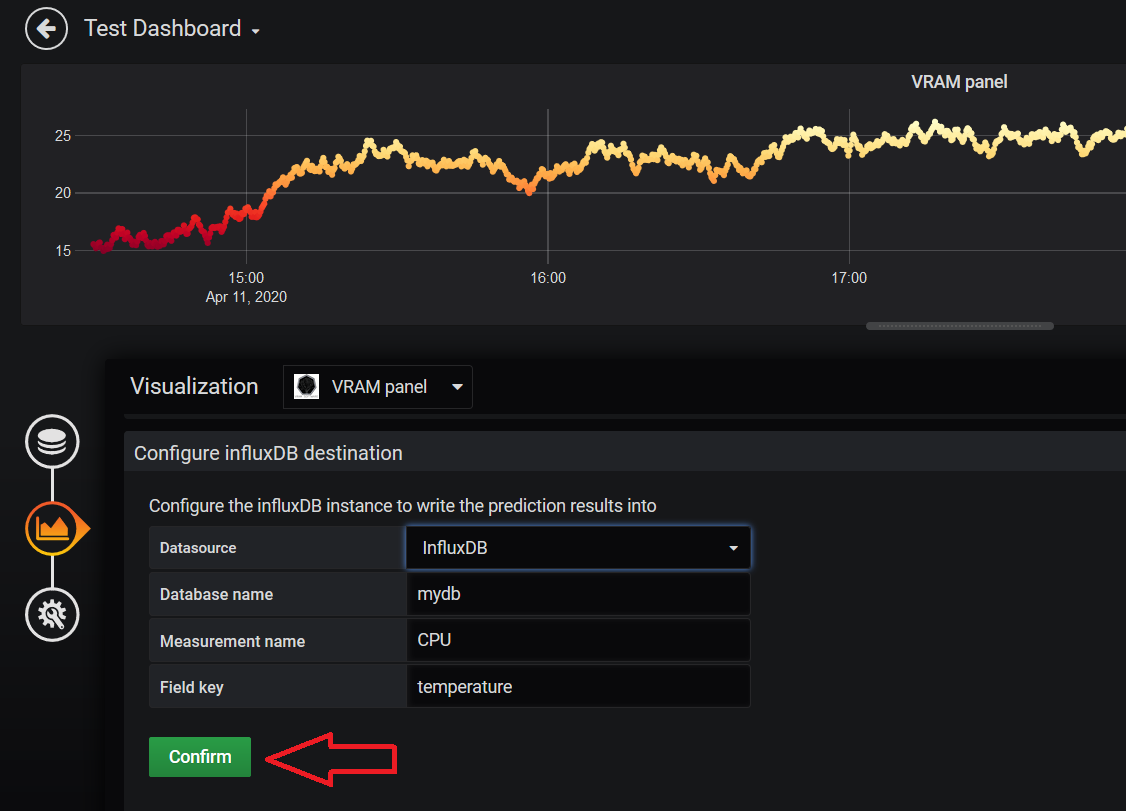
\includegraphics[width=\textwidth,height=\textheight,keepaspectratio]{img/scrittura_InfluxDB.png}
            \caption{Riquadro "Configure influxDB destination".}
        \end{figure}
    \subsection{Modifiche di visualizzazione del grafico}
        Infine sono presenti due riquadri ("Display" e "Traces") e una toolbar nel grafico tramite i quali è possibile modificare l'aspetto del grafico utilizzando varie opzioni come ad esempio l'aggiunta di tracce che possono evidenziare altre query inserite.
        \begin{figure}[H]
            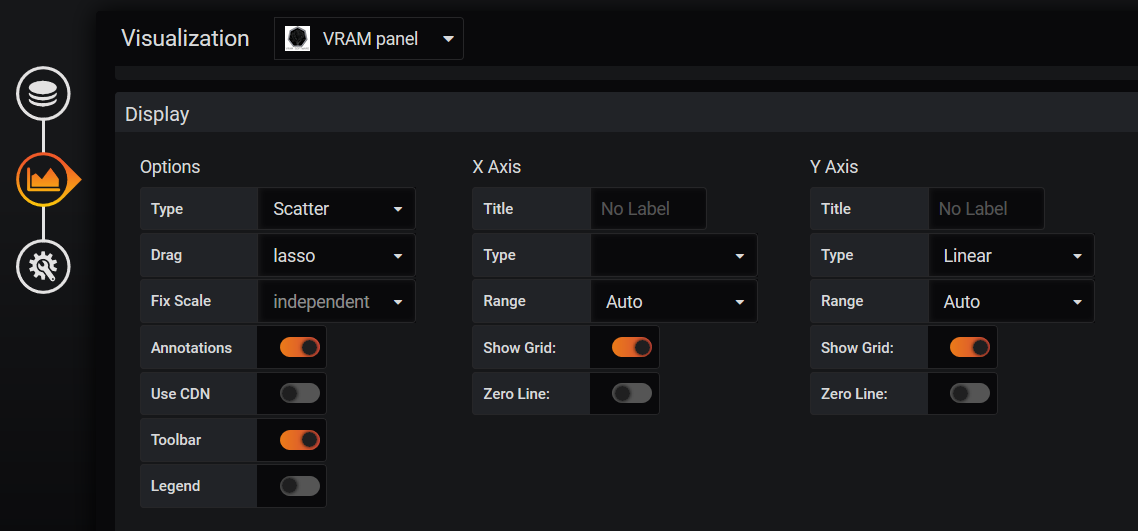
\includegraphics[width=\textwidth,height=\textheight,keepaspectratio]{img/display.png}
            \caption{Riquadro "Display".}
        \end{figure}
        \begin{figure}[H]
            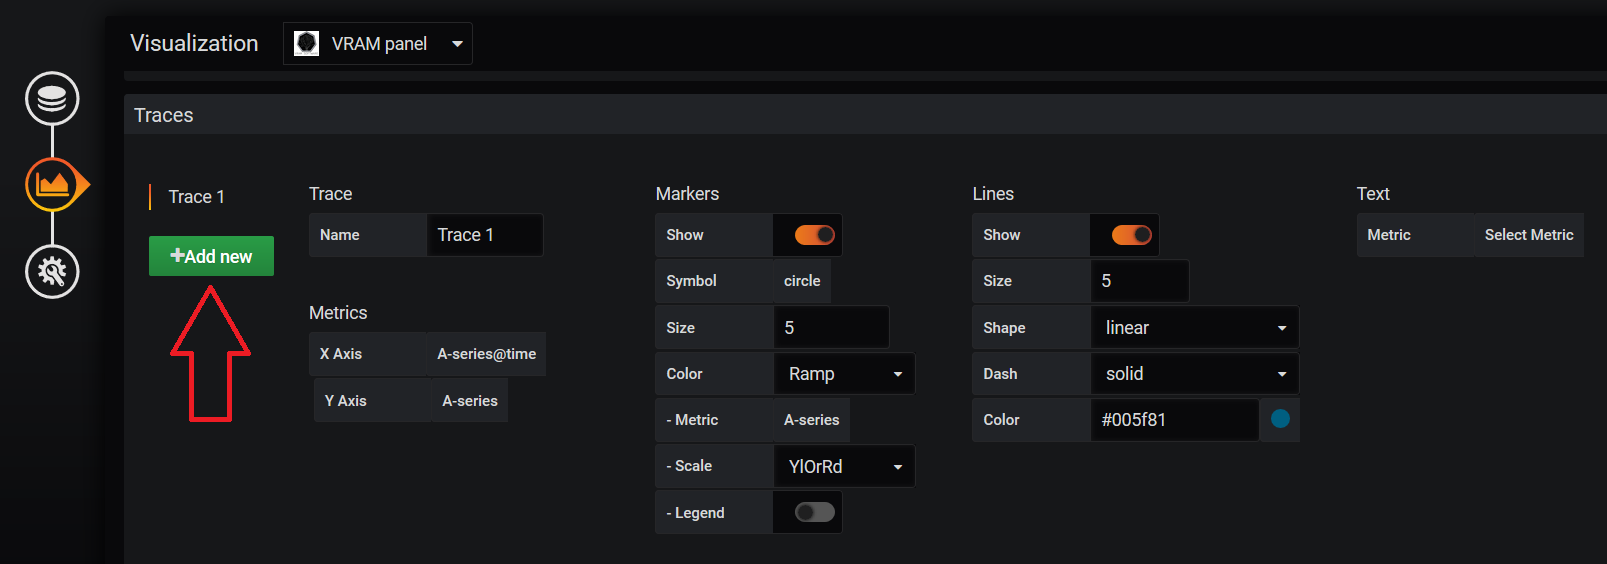
\includegraphics[width=\textwidth,height=\textheight,keepaspectratio]{img/traces.png}
            \caption{Riquadro "Traces".}
        \end{figure}
        \begin{figure}[H]
            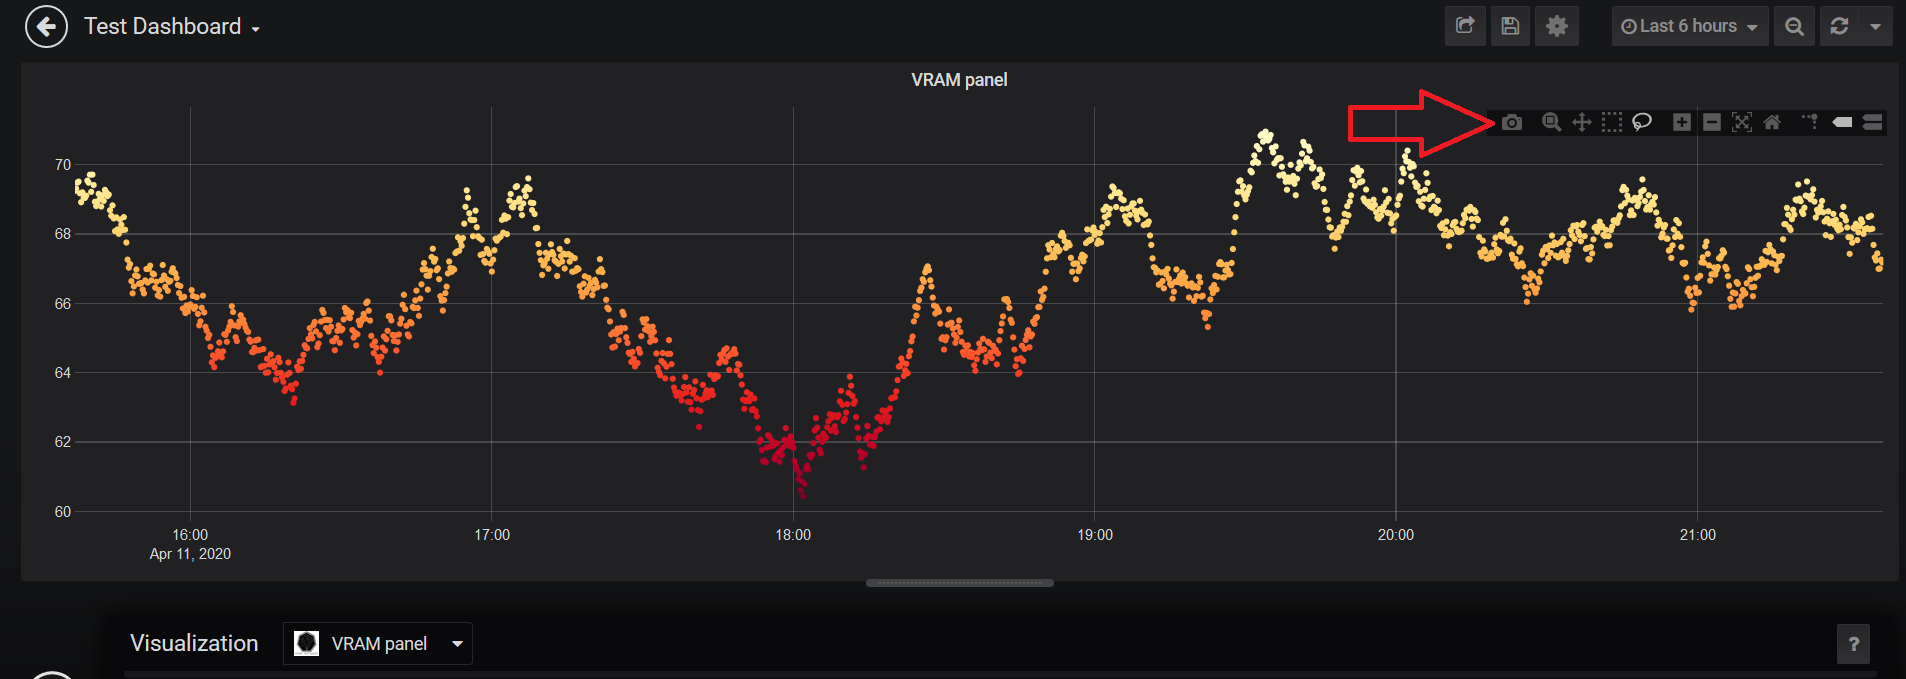
\includegraphics[width=\textwidth,height=\textheight,keepaspectratio]{img/toolbar.png}
            \caption{Toolbar inserita nel grafico.}
        \end{figure}